\section{Punainen nahkalilja 5.10.}\label{section:punainenNahkalilja}

\begin{multicols}{2}
\noindent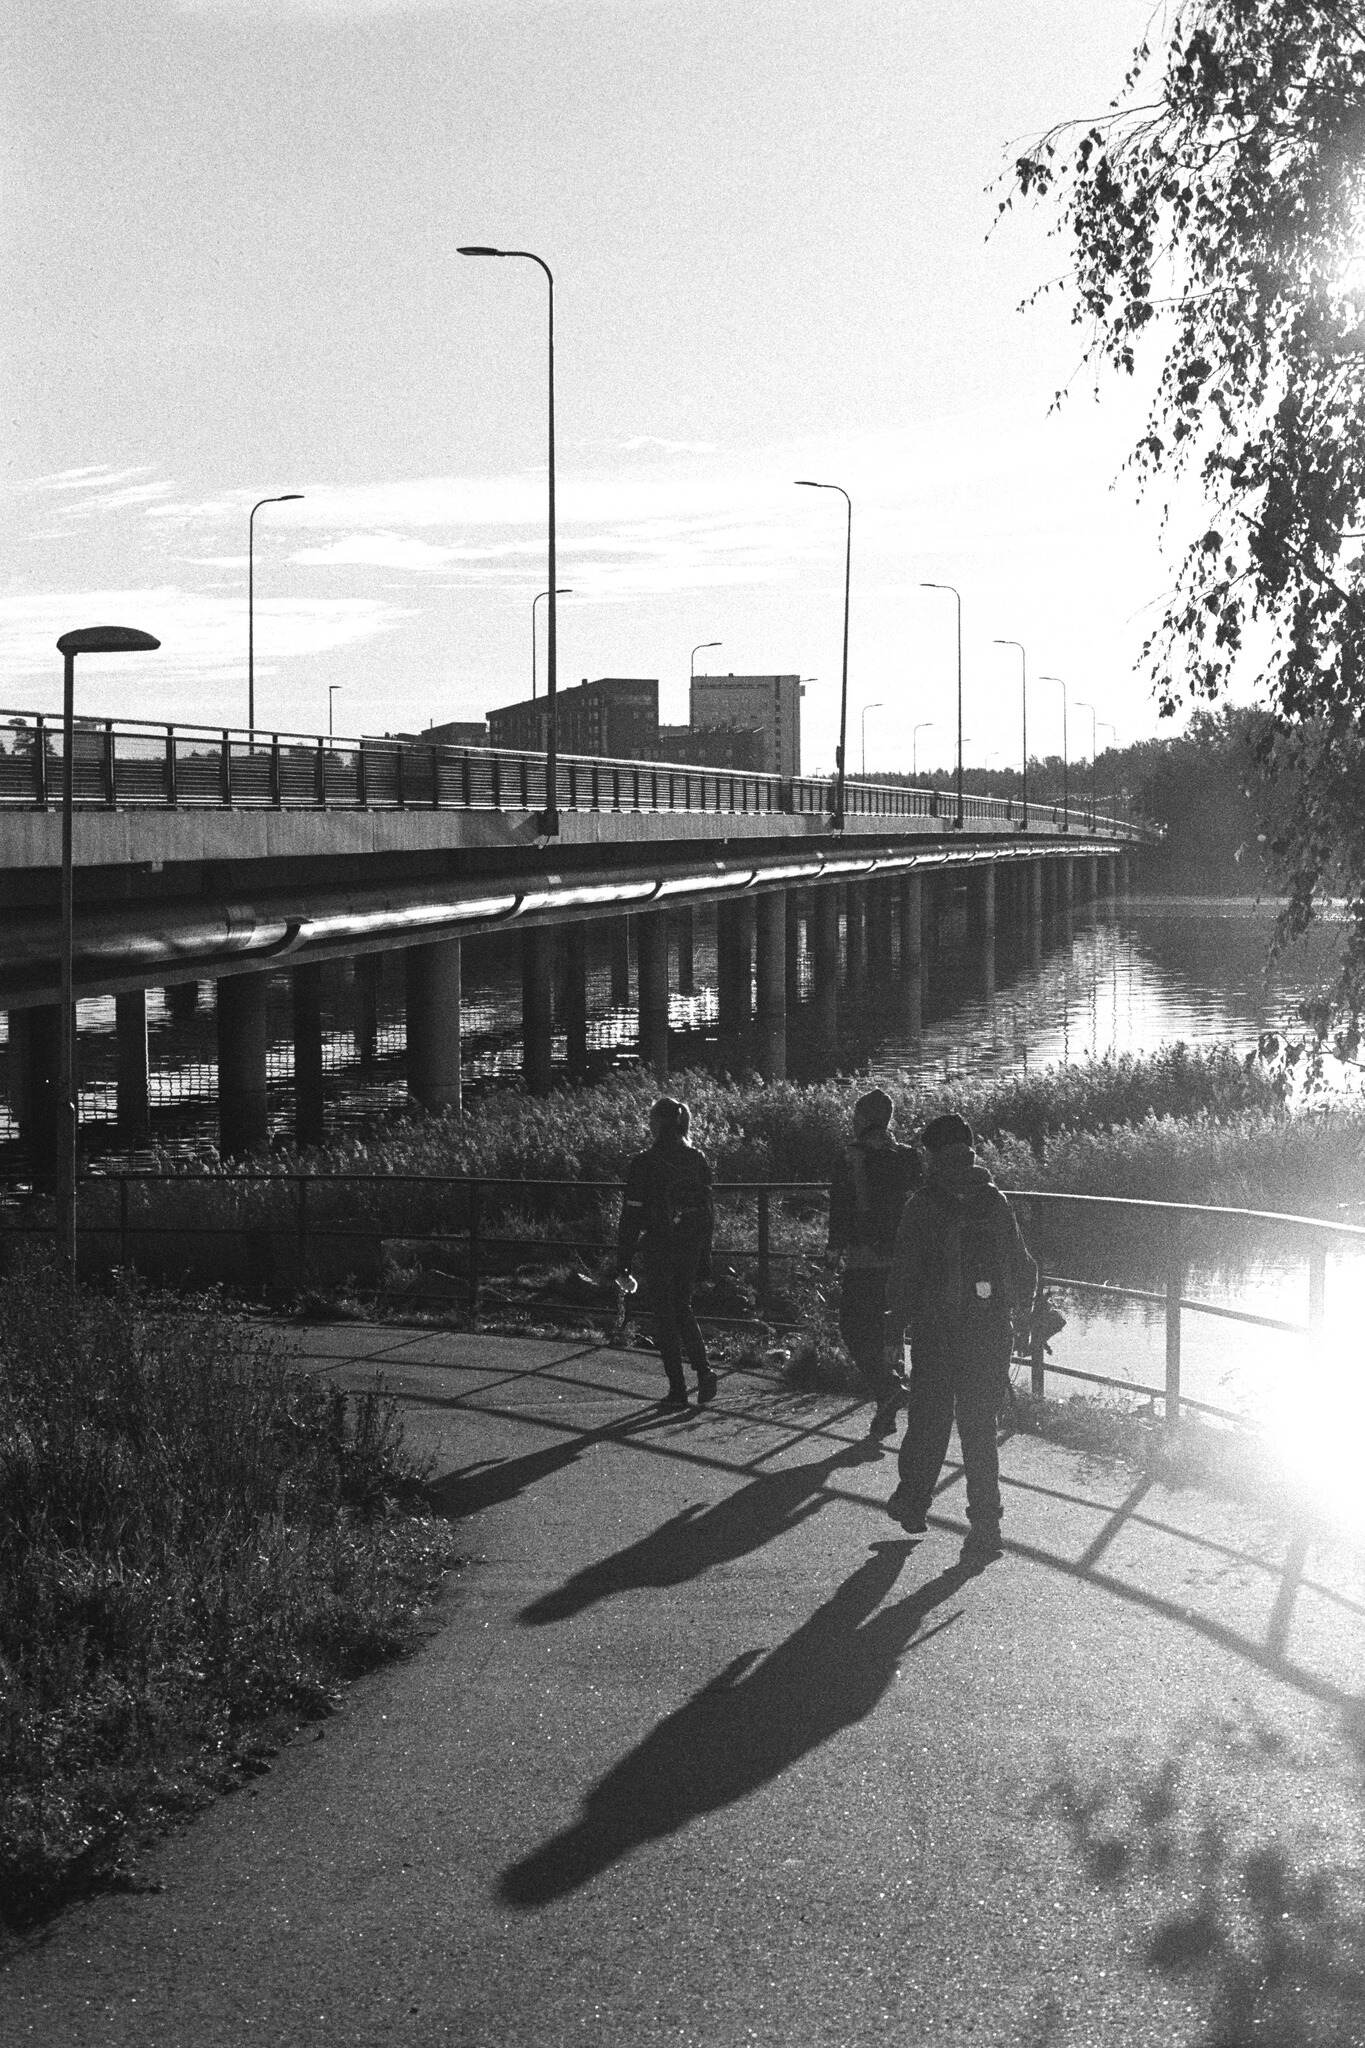
\includegraphics[width=\linewidth,trim={0 3cm 0 6.75cm},clip]{assets/nahkaliljapunainen1.jpg}

\vfill

\noindent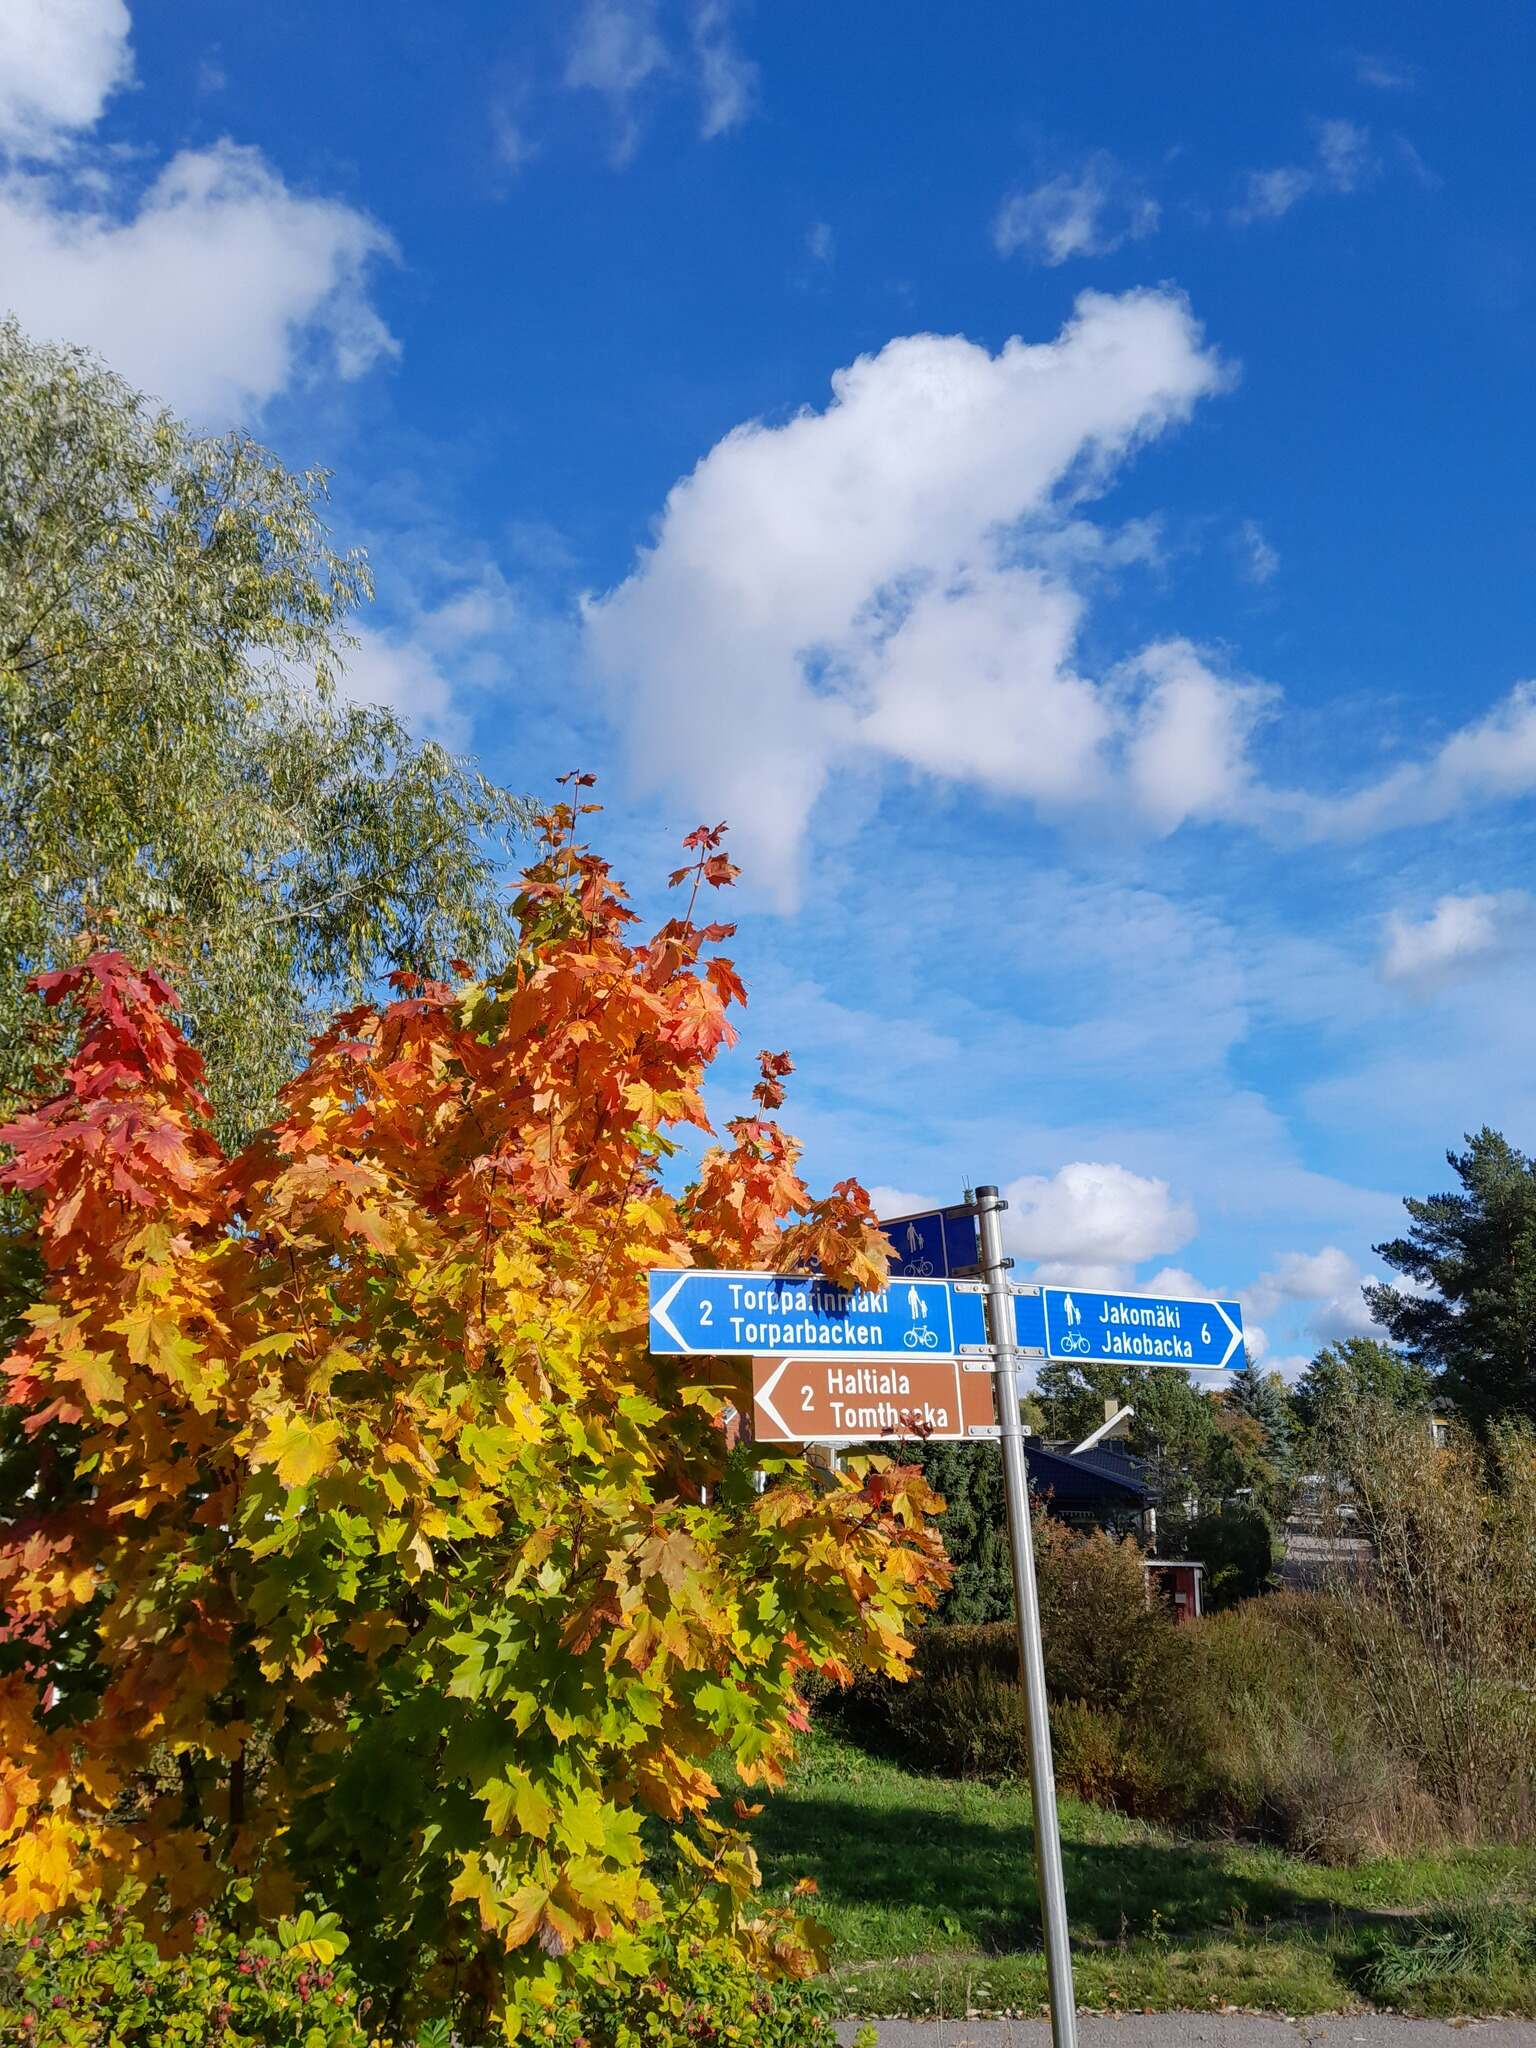
\includegraphics[width=\linewidth,trim={0 0 0 2cm},clip]{assets/nahkaliljapunainen2.jpg}

\columnbreak

\noindent Lokakuun viides päivä, syksyllä 2024 Kontulan Mikaelinkirkon 
edustalta lähti neljä rusakkoa suorittamaan punaista nahkaliljaa. Kaikki 
neljä olivat paikalla viittä yli kahdeksan, jolloin matkalle lähdettiin. 

Matka alkoi suuntaamalla kaakkoon kohti Vartiokylänlahtea. Ensimmäinen tauko 
pidettiin Vartiokylänlahden sillan kupeessa lahden itäpuolella, joka oli 
reitin eteläisin kohta, jota hieman ennen oltiin kävelty reitin itäisimmän 
kohdan eli lahden pohjoispään ohi. Siitä matkaa jatkettiin sillan yli ja 
Itäkeskuksen kautta takaisin kirkolle. Näin saatiin täyteen kymmenen 
kilometrin lenkki, jonka jälkeen matkaan mukaan otettiin myös kymmenen 
kilometriä lyhyemmän, vihreän nahkaliljan yksi suorittaja sekä sata 
kilometriä pitkän mustan nahkaliljan suorittaja. 

Kirkolla pidettiin samalla myös matkan toinen tauko ennen kuin matkaa 
jatkettiin pohjoiseen Rajakylään ja siitä länteen kohti Jakomäkeä. 
Seivästien pysäkillä pidettiin myös aikataulusta poiketen tauko, koska yksi 
rusakoista oli unohtanut huivinsa kotiin ja kävi sen hakemassa. Jakomäestä 
matka jatkui länteen neljännelle tauolle Tapulikaupunkiin Mosan 
jalkapallokentälle.

Pallokentältä lähdettyään rusakot jatkoivat länteen Tapaninkylän läpi 
Tammistoon. Vantaanjoen rannalla pidettiin tauko, jonka jälkeen matka jatkui 
joen rantaa vastavirtaan, eli pohjoiseen kohti Pakkalaa, jossa reitiltä 
poikettiin kauppaan evästauolle, joka merkkasi punaisen liljan suorittajille 
matkan puoliväliä.

Pakkalasta matka jatkui länteen Ylästön läpi kohti Silvolan tekojärveä, 
jota ennen oli reitin pohjoisin kohta ja jonka läntisellä rannalla oli reitin 
läntisin kohta. Tekojärvellä rusakko"-osasto myös jakautui kahtia, kun 
mustan ja vihreän liljan suorittajat mukanaan yksi punaisen liljan 
suorittajista teki irtioton muista punaisen liljan suorittajista, koska mustan 
liljan aikaraja alkoi tulla vastaan. 

Silvolasta reitti jatkui etelään Vantaanjoen yli ja Keskuspuiston läpi. 
Edellä olevat rusakot pitivät Keskuspuistossa matkan seitsemännen tauon. 
Keskuspuistosta poistumisen jälkeen oli reitillä vuorossa matkan kymmenes 
silta, joka oli pikaratikan raiteet ylittävä silta Maunulassa. Maunulan 
ulkoilumajalla pitivät etujoukot tauon, jolloin osa rusakoista söi eväänsä 
loppuun.

Maunulasta matka jatkui itään Metsälän läpi ja Käpylän juna"-aseman ohi 
Taivaskalliolle, jossa edellä menevät rusakot pitivät tauon. Taivaskalliolta 
matka jatkui taas itään. Rusakot siirtyivät Vanhankaupunginkoskella takaisin 
Vantaanjoen itäpuolelle. Edellä menevät rusakot seurasivat suunniteltua 
reittiä Viikin arboretumin läpi, kun takaa tulevat rusakot päättivät 
oikaista ja mennä Viikintien suoraa pitkin. Musta lilja irtosi vielä 
arboretumin jälkeen Mäyrämetsässä pidetyllä tauolla muusta etujoukosta ja 
lopetti suorituksensa kello 19.35 Siilitielle.

Tässä vaiheessa vihreä lilja ja yksi punaisen suorittajista jäi jo muun 
punaisen liljan tekemän oikaisun takia jälkeen. Punainen lilja käveli 
Siilitien, Myllypuron ja Kontulan läpi takaisin maaliin kirkolle, jossa se oli 
noin kello 20.27. Vihreä lilja lopetti suorituksensa Myllypuron metroasemalle 
kello 20.39, josta punaisen liljan viimeinen osio käveli vielä kirkolle 
maaliin, jossa se oli kello 20.58.

\vspace*{.25cm}

\noindent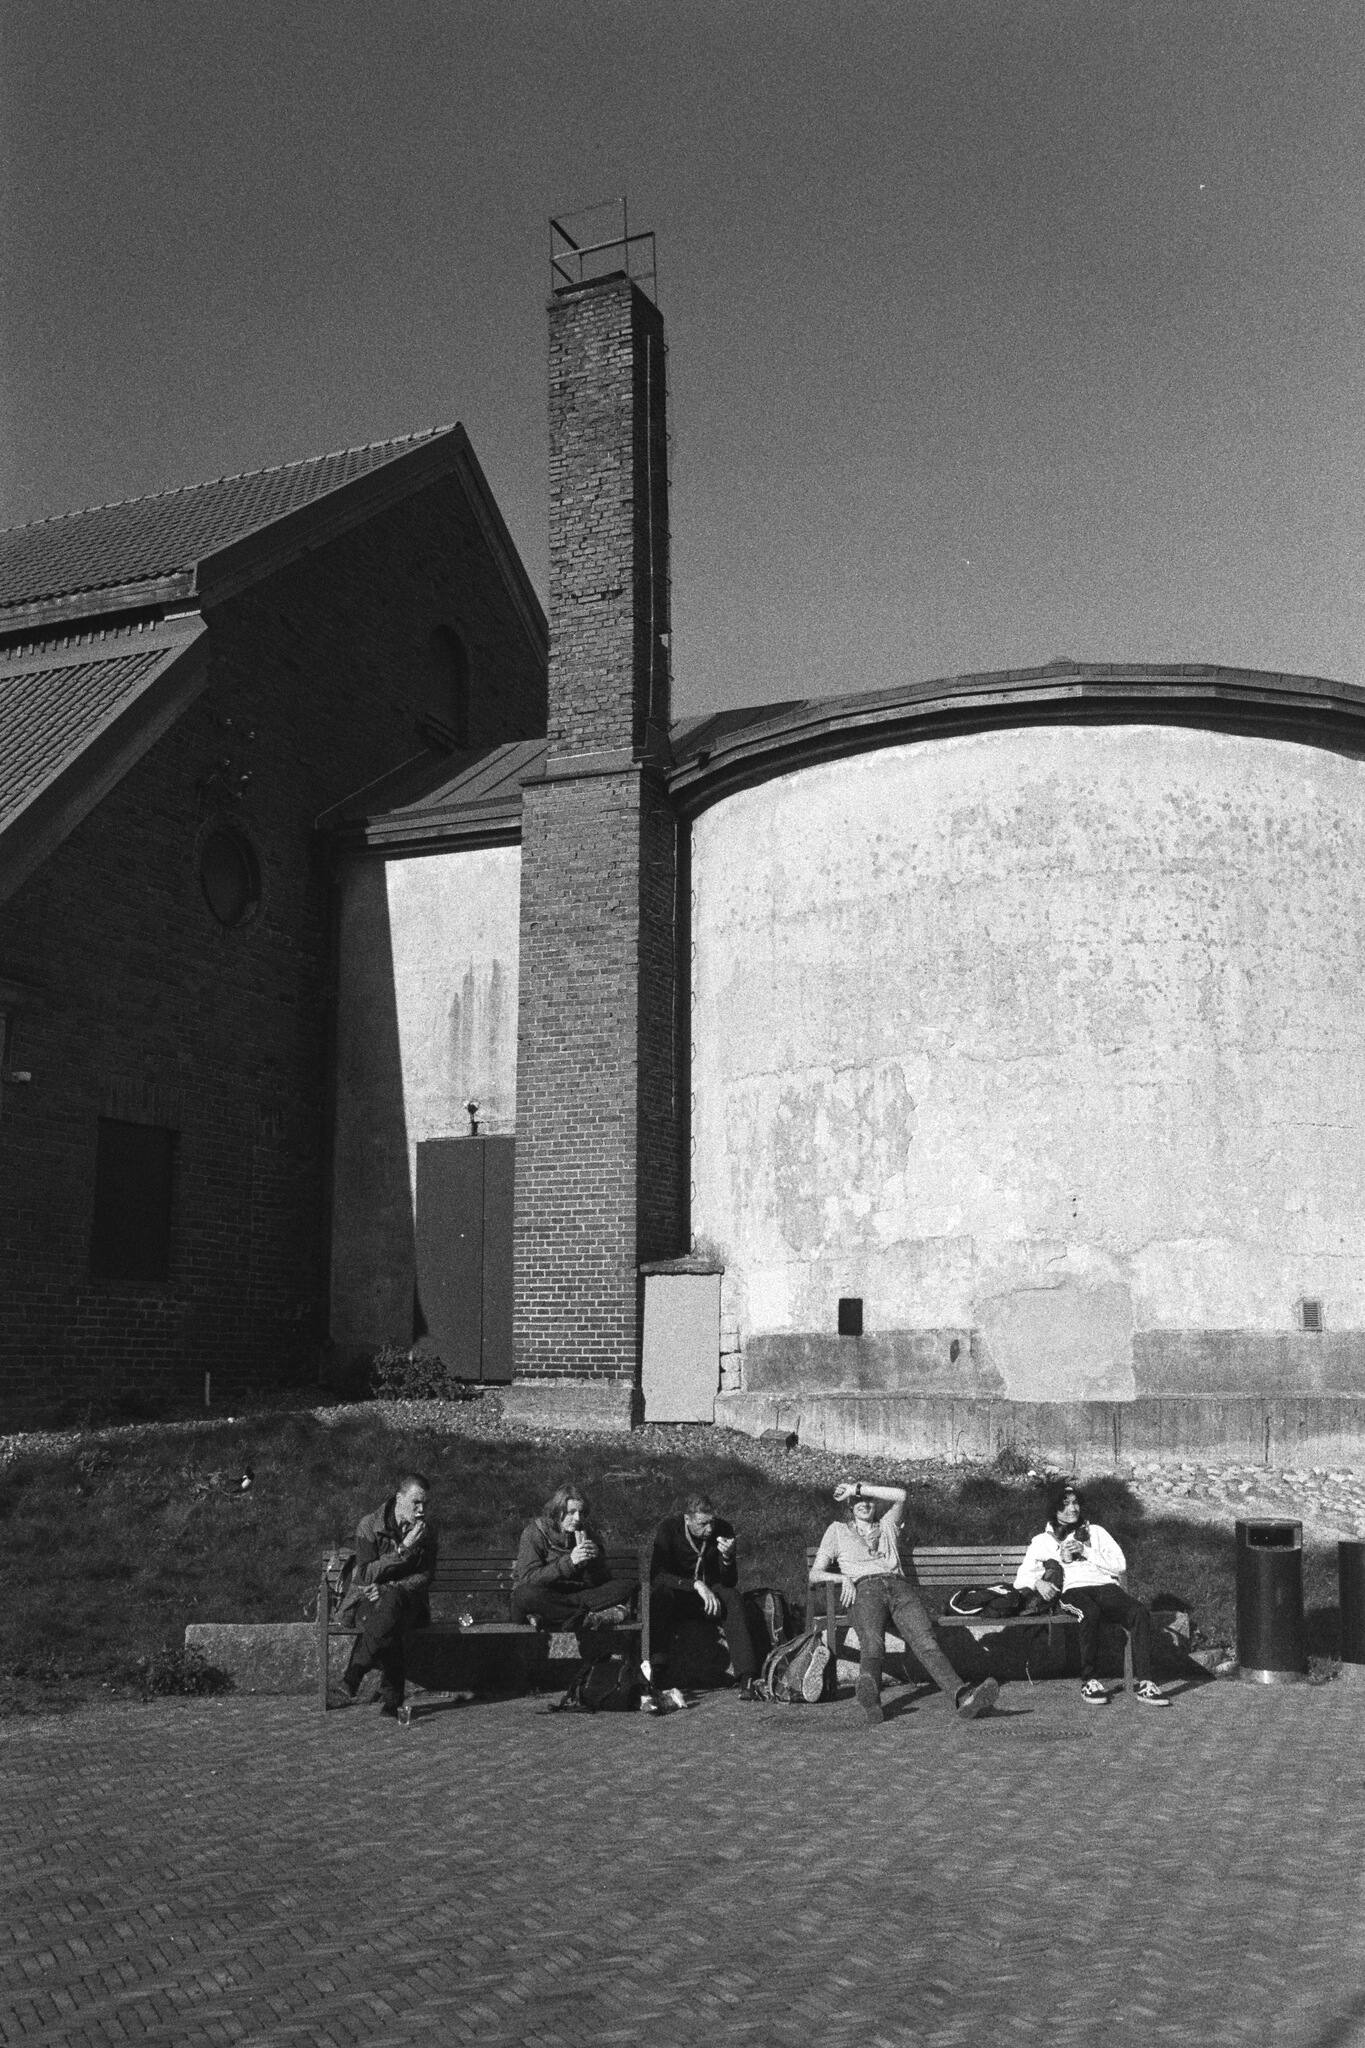
\includegraphics[width=\linewidth]{assets/nahkaliljapunainen3.jpg}

\vspace*{.25cm}

{\raggedleft Kuvat: Tanguy Gérôme\\Teksti: Ahti Niinimäki\par}
\end{multicols}
